\documentclass[twoside,11pt]{article}
\PassOptionsToPackage{hyphens}{url}
\usepackage{jmlr2e}
\usepackage{amsmath}
\usepackage[toc,page]{appendix}
\usepackage[table]{xcolor}
\usepackage[marginparsep=30pt]{geometry}
\usepackage{stmaryrd}
\usepackage{algorithm}
\usepackage{algorithmic}
\usepackage{tikz}
\usepackage{pgfplots}
\usepackage{tabu}
\usepackage{longtable}
\usepackage{tabularx}
\usepackage{listings}
\usepackage{fancyref}
\usepackage{relsize}
\usepackage{float}
\usepackage{subcaption}

\usetikzlibrary{%
    arrows,
    arrows.meta,
    decorations,
    backgrounds,
    positioning,
    fit,
    petri,
    shadows,
    datavisualization.formats.functions,
    calc,
    shapes,
    shapes.multipart,
    matrix,
    plotmarks
}

\usepgfplotslibrary{fillbetween, statistics}

\pgfplotsset{
  compat=1.3,
  every non boxed x axis/.style={
  enlarge x limits=false,
  x axis line style={}%-stealth},
  },
  every boxed x axis/.style={},
  every non boxed y axis/.style={
  enlarge y limits=false,
  y axis line style={}%-stealth},
  },
  every boxed y axis/.style={},
}

\def\perc{\texttt{perco\-late}}
\def\v{\texttt{v0.1.0}}

\def\titl{Message Passing Programming coursework:
  optimization of \perc{} \v{} using a 2d domain
  decomposition with MPI}

\title{\titl}

\author{}

\ShortHeadings{B160509}{B160509}
\firstpageno{1}


\begin{document}

\maketitle

\begin{abstract}
\end{abstract}

\begin{keywords}
Scientific programming, benchmark, parallelization,
performance optimization, MPI
\end{keywords}

\section{Introduction} % {{{

\perc{} \v{} is a scientific program written in the Fortran
programming language. It generates a random matrix with two
kinds of cells: empty and filled. Empty cells build
clusters with their neighboring empty cells.
\perc{} computes all clusters in the matrix and searches
for a cluster that makes the matrix percolate.
The matrix percolates, if there exits a cluster that begins
in the left most column of the matrix and ends in the right
most column.

The computing of the clusters---the clustering---is done
iteratively and is the main cause of computation in
\perc{}.
If the clustering is done in a serial way, it does not
scale well and clustering bigger matrices can consume a
lot of time and power.

This paper presents a parallelized version of \perc{}.
The parallel version decomposes the matrix into smaller
chunks and distributes them among worker instances.
Every worker performs the clustering of its chunk and
communicates with the neighboring worker
instances through halo swapping, which ensures that the
whole matrix is clustered.
Chunks are generated by splitting the matrix on both axes.
This makes it a 2d domain decomposition of the matrix.
The parallel version is based on MPI and the worker
instances are MPI processes \citep[see][]{mpi}.

First, this paper describes the clustering algorithm used
by \perc{} and the way \perc{} is parallelized using the
MPI library.
The parallel version's correctness is tested by a
regression test suite, which is briefly outlined.
Afterwards a benchmark is presented, which analyzes the
scaling behavior of the parallel version over multiple
amounts of MPI processes and with different sized matrices.
The results of the benchmark are discussed and a conclusion
is drawn.

% }}}

\section{Method} % {{{

This chapter presents a mathematical definition of the
clustering algorithm used by \perc{}.
The poor running time of the serial version of the
clustering algorithm is shown.
Afterwards the parallelized version of the clustering is
described and a brief outline of the regression test suite
for testing the correctness of the parallel version is
given.
At last, this chapter presents the benchmark, that is
discussed in the following chapters.

% math def {{{

\subsection{Mathematical definition of the clustering
  algorithm used by \perc{}}

Let $A \in \mathbb{N}_0^{n \times n}$ be the matrix that
is clustered by \perc{}.
Let $A(i, j);1\leq i, j \leq n$ be the element at the
$i$th row and $j$th column of $A$.
An element from $A$ has a state. It is either empty or
filled.
\perc{} randomly initializes $A$ with empty and filled
elements.
The density of the filled elements $\rho_{goal}$ can be
defined as a parameter, which is approximated during
initialization. $n$, as well, is provided as a parameter to
\perc{}.

Let $\sigma : \mathbb{N}_0 \rightarrow \{empty,filled\}$ be
a function mapping a non-negative integer to its state:
\begin{align*}
  \sigma(x) := \begin{cases}
    filled &\text{if } x = 0 \\
    empty  &\text{otherwise}
  \end{cases}.
\end{align*}

\begin{proposition}
  \label{prop:one}
  Let $x, y \in \mathbb{N}_0$.
  For every $x: \sigma(x) = empty$, follows: $x > y$, if
  $\sigma(y) = filled$.
\end{proposition}

\begin{proof}
  There exits no smaller non-negative integer than $0$.
  $\sigma(y) = filled$, only for $y = 0$. Therefore, every
  number $x$, for which $\sigma(x) = empty$, must be bigger
  than $y$.
\end{proof}

Let $\mu$ be the function that returns the maximum value
of an element and its neighbors:
\begin{align*}
  \mu(A, i, j) := \max(A(i,j), A(i-1,j), A(i+1,j),
                       A(i,j-1), A(i,j+1)).
\end{align*}
For now, if $i$ or $j$ equals $0$ or $n + 1$ (in other
words, if $i$ or $j$ violate the boundaries of $A$), then
$A(i, j)$ will return $0$.

\begin{proposition}
  \label{prop:two}
  If $\sigma(A(i, j)) = empty$, than
  $\sigma(\mu(A, i, j)) = empty$ as well.
\end{proposition}

\begin{proof}
  $\mu(A, i, j)$ returns the maximum of the element
  $A(i, j)$ and its neighbors, wherefore $\mu(A, i, j) \geq
  A(i, j)$.
  From Proposition~\ref{prop:one} follows, that every
  number $y \in \mathbb{N}_0: \sigma(y) = filled$ must be
  less than $A(i, j)$, if $\sigma(A(i,j)) = empty$.
\end{proof}

With Proposition~\ref{prop:two}, we can now safely derive
a recursive definition of the clustering operation (because
$\mu$ will never change the state of an empty cell to
filled).
First, let $c_{step}:\mathbb{N}_0^{n \times n} \rightarrow
\mathbb{N}_0^{n \times n}$ be a single clustering step,
that maps every empty element of $A$ to its biggest
neighbor and leaves filled elements untouched:
\begin{align*}
  c_{step}(A) := i,j=1,\dots,n: \begin{cases}
    \mu(A, i, j) &\text{if } \sigma(A(i, j)) = empty \\
    0 &\text{otherwise}.
  \end{cases}
\end{align*}
The clustering operation $c$ of \perc{} can now be defined
as a recursive function, that executes $c_{step}$, as long
as it continues to change empty elements to their biggest
neighbor:
\begin{align*}
  c(A) := \begin{cases}
    A &\text{if } c_{step}(A) = A \\
    c(c_{step}(A)) &\text{otherwise}.
  \end{cases}
\end{align*}

Imagine the case where for every element
$\sigma(A(i,j)) = filled$ follows, that
$\mu(A, i, j) = A(i, j)$.
This would make $c(A)$ call $c_{step}$ just a single time,
resulting in the best case running time of $c$:
$\Omega(c) = n^2$, which---for bigger $n$---is still quite
slow, even though it is the best case.

After the clustering, it is easy to check whether the
matrix percolates.
The matrix percolates, if $\exists i, \exists j: A(i,1) =
A(j,n)$.
In other words, if any element in the first column has the
same value as any element in the last column of $A$, the
matrix percolates.

% }}}

% parallel {{{

\subsection{Parallelized version of \perc{} using MPI}

To tackle the poor performance of the clustering algorithm,
\perc{} was parallelized using the MPI Standard,
version 3.1 \citep[see][]{mpi}.

Let $p$ be the amount of MPI processes the parallel version
of \perc{} is executed with.
Every process has a rank, which is drawn from a sequence
$0,1,\dots,p-1$.
The process with rank 0 is called the root process.

The processes are arranged in a virtual, two dimensional
Cartesian topology.
The $p$ processes are as evenly distributed as possible
over both axes of the topology with the
\texttt{MPI\_Dims\_create} routine.
\texttt{MPI\_Dims\_create} returns an array $dims$ with two
elements, one for each axis.
$dims_{row}$ contains the amount of processes the rows of
$A$ are split by, $dims_{column}$ the amount of processes
the columns of $A$ are split by.
After generating the dimensions of the topology,
\texttt{MPI\_Cart\_create} is used to generate the actual
communicator that manages the virtual topology with
\texttt{MPI\_Comm\_World} \citep[see][Chapter 7]{mpi}.

The previous chapter states, that $A(i, j) = 0$, if $i$ or
$j$ equals $0$ or $n + 1$ ($i$ or $j$ out of bounds).
The actual clustering of \perc{} behaves differently.
$A(i, j) = 0$, only if $j$ is out of bounds.
If $i$ is out of bounds, then a periodic boundary condition
is used: $A(0, j) = A(n, j), A(n + 1, j) = A(1, j)$.
This condition is easily implemented with
\texttt{MPI\_Cart\_create}, which actually has an argument
\texttt{periods}. \texttt{periods} is an array with two
elements (for each axis) containing boolean values, whether
an axis of the topology is periodic or not
\citep[see][Chapter 7]{mpi}.

The root process initializes $A$, which needs to be
distributed to the MPI processes.
Every process has coordinates in the topology, based on
its rank.
The coordinates of a process come from the
\texttt{MPI\_Cart\_coords} routine and are a representation
of the place of the process in the two dimensional
Cartesian topology \citep[see][Chapter 7]{mpi}.

Let $coords_{p_i}$ be the coordinates of the process with
rank $p_i$ and let $coords_{p_i, row}$ be the coordinates'
value for the first axis and $coords_{p_i, column}$ be its
value for the second axis of the topology.
$coords$ behaves like the ranks, ranging from $0$ to
$dims_{row} - 1$ and $0$ to $dims_{column} - 1$,
respectively \citep[see][Chapter 7]{mpi}.

The chunk of $A$, which is assigned to the process with
rank $p_i$ can now be defined by a tuple
$\alpha_{p_i} := (i, j, l, m)$.
$i$ and $j$ are the indices of $A$, which point to the
first element of the chunk, while $l$ is the amount of rows
and $m$ the amount of columns the chunk possesses.
Let $s_{row} := \lfloor \frac{n}{dims_{row}} \rfloor$ and
$s_{column} := \lfloor \frac{n}{dims_{column}} \rfloor$ be
the general size of the splits of $A$ for both axes.
With use of these split values and $coords$ and $dims$, we
can define $i, j, l$ and $m$:
\begin{align*}
  &i := coords_{p_i,row} \cdot s_{row} + 1 \\
  &j := coords_{p_i, column} \cdot s_{column} + 1 \\
  &l := \begin{cases}
    s_{row} + n \mod dims_{row} &\text{if } coords_{p_i, row} = dims_{row} - 1 \\
    s_{row} &\text{otherwise}
  \end{cases} \\
  &m := \begin{cases}
    s_{column} + n \mod dims_{column} &\text{if } coords_{p_i, column} = dims_{column} - 1 \\
    s_{column} &\text{otherwise}.
  \end{cases}
\end{align*}
For both axes of $A$, every process has a chunk of the same
size, except the processes, which coordinates' value for
the equivalent axis in the topology is the highest possible
value for it ($dims_{row} - 1$ or $dims_{column} - 1$).
The last process has a chunk of the same size as the other
processes, plus the rest of the elements of $A$ among that
axis.

% exception if dims_xxx > L

$l$ and $m$ are needed in order to generate a strided
vector type with \texttt{MPI\_Type\_vector}, which is used
for sending the chunk from the root process to $p_i$.
In this case, the type for sending $p_i$'s chunk would be
generated with setting \texttt{count} to $m$,
\texttt{blocklength} to $l$ and \texttt{stride} to $n$
\citep[see][Chapter 4]{mpi}.

% here chunks

% scatter/gathering at the root process

% scatter gather

% neighbors

% halo swap

% example

% graph with example of splitting map
\begin{figure}
\begin{subfigure}[t]{\textwidth}
\begin{center}
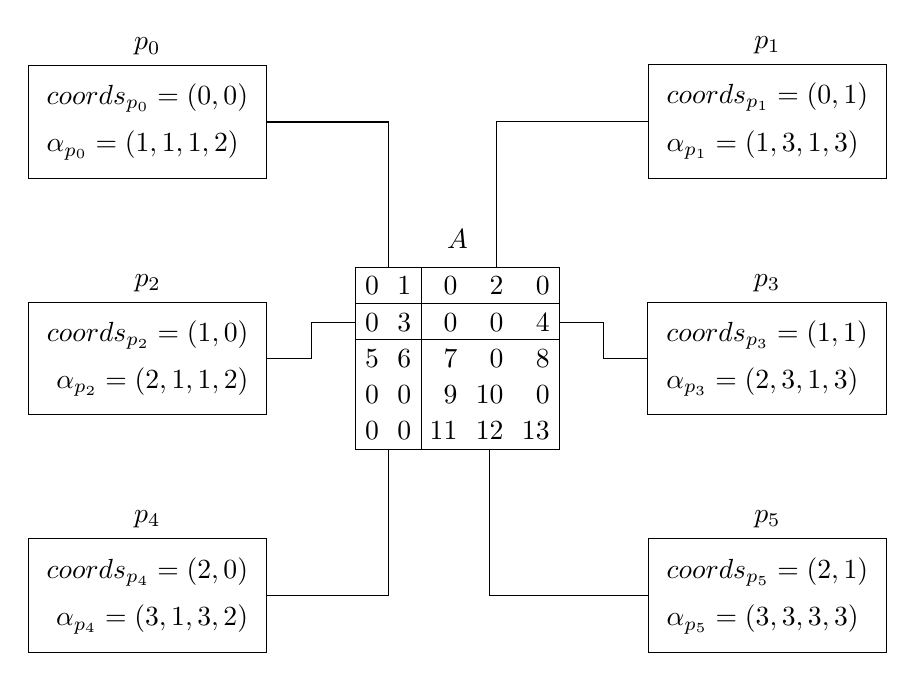
\begin{tikzpicture} % {{{
  \matrix[anchor=east, label=$A$]
  at (0, 0) (A)
  {
    \node (ps)   {0}; & \node (pvs) {1}; & \node        {0};
                      & \node (pp1) {2}; & \node        {0}; \\
    \node (ph1s) {0}; & \node       {3}; & \node        {0};
                      & \node       {0}; & \node (ph1e) {4}; \\
    \node (ph2s) {5}; & \node       {6}; & \node        {7};
                      & \node       {0}; & \node (ph2e) {8}; \\
    \node        {0}; & \node       {0}; & \node        {9};
                      & \node      {10}; & \node        {0}; \\
    \node (pp4)  {0}; & \node (pve) {0}; & \node       {11};
                      & \node (pp5){12}; & \node (pe)  {13}; \\
  };

  \draw (ps.north west) -| (pe.south east) -| cycle;
  \draw (ph1s.north west) -- (ph1e.north east);
  \draw (ph2s.north west) -- (ph2e.north east);
  \draw (pvs.north east) -- (pve.south east);

  \matrix[above left=1.42cm of A.north west, label=$p_0$, draw] (p0)
  {
    \node[anchor=west]{$coords_{p_0} = (0, 0)$};\\
    \node[anchor=west]{$\alpha_{p_0} = (1, 1, 1, 2)$};\\
  };

  \matrix[above right=1.42cm of A.north east, label=$p_1$, draw] (p1)
  {
    \node{$coords_{p_1} = (0, 1)$};\\
    \node{$\alpha_{p_1} = (1, 3, 1, 3)$};\\
  };
  \matrix[left=1cm of A.west, label=$p_2$, draw] (p2)
  {
    \node{$coords_{p_2} = (1, 0)$};\\
    \node{$\alpha_{p_2} = (2, 1, 1, 2)$};\\
  };
  \matrix[right=1cm of A.east, label=$p_3$, draw] (p3)
  {
    \node{$coords_{p_3} = (1, 1)$};\\
    \node{$\alpha_{p_3} = (2, 3, 1, 3)$};\\
  };
  \matrix[below left=1.42cm of A.south west, label=$p_4$, draw] (p4)
  {
    \node{$coords_{p_4} = (2, 0)$};\\
    \node{$\alpha_{p_4} = (3, 1, 3, 2)$};\\
  };
  \matrix[below right=1.42cm of A.south east, label=$p_5$, draw] (p5)
  {
    \node{$coords_{p_5} = (2, 1)$};\\
    \node{$\alpha_{p_5} = (3, 3, 3, 3)$};\\
  };

  \draw (p0) -| (ps.north east);
  \draw (p1) -| (pp1);
  \draw (p2) -| ($(p2.east) !.5! (ph1s.west)$) |- (ph1s);
  \draw (p3) -| ($(p3.west) !.5! (ph1e.east)$) |- (ph1e);
  \draw (p4) -| (pp4.south east);
  \draw (p5) -| (pp5);
\end{tikzpicture} % }}}
\caption{Subfig}
\end{center}
\vspace{2cm}
\end{subfigure}
\begin{subfigure}[t]{\textwidth}
\begin{center}
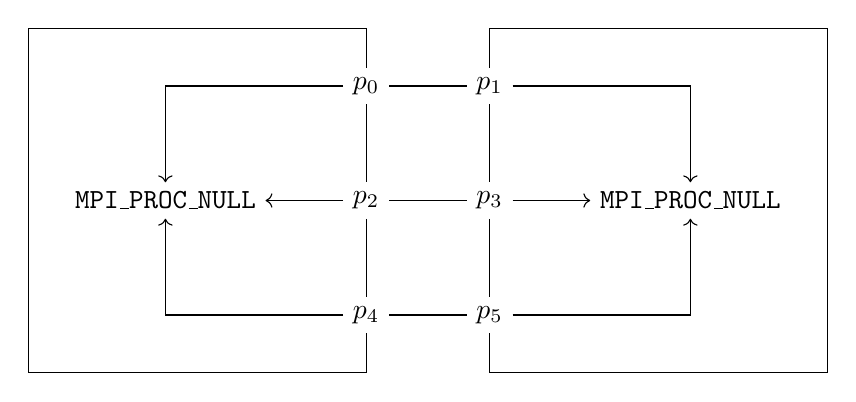
\begin{tikzpicture} % {{{
  \matrix[column sep=1cm, row sep=1cm]{
    &\node (p0) {$p_0$}; &\node (p1) {$p_1$}; &\\
    \node (nullw)  {\texttt{MPI\_PROC\_NULL}};
    &\node (p2) {$p_2$}; &\node (p3) {$p_3$};
      &\node (nulle) {\texttt{MPI\_PROC\_NULL}}; \\
    &\node (p4) {$p_4$}; &\node (p5) {$p_5$}; \\
  };

  \draw[->] (p0) -| (nullw);
  \draw[->] (p2) -- (nullw);
  \draw[->] (p4) -| (nullw);

  \draw[-] (p0) -- (p2);
  \draw[-] (p2) -- (p4);

  \draw[-] (p0) -- (p1);
  \draw[-] (p4) -- (p5);

  \draw[->] (p1) -| (nulle);
  \draw[->] (p3) -- (nulle);
  \draw[->] (p5) -| (nulle);

  \draw[-] (p1) -- (p3);
  \draw[-] (p3) -- (p5);

  \draw[-] (p2) -- (p3);

  \draw[-] (p0) |- ($(p0.north west) + (-4cm,.5cm)$) --
             ($(p4.south west) - (4cm,.5cm)$) -| (p4);

  \draw[-] (p1) |- ($(p1.north east) + (4cm,.5cm)$) --
             ($(p5.south east) + (4cm,-.5cm)$) -| (p5);

\end{tikzpicture} % }}}
\caption{Subfig, TODO: describe directed graph property}
\end{center}
\end{subfigure}
\caption{Fig}
\label{fig:example}
\end{figure}

In order to insure correctness of the result, the first
axis of the topology can not contain more elements than $n$
($dims_{row} \leq n$), because this axis uses a periodic
boundary condition.
If $dim_{row} > n$, than $s_{row} = 0$. That means, only
the processes with $coords_{row} = dims_{row} - 1$ would
contain elements and all other processes would contain
empty chunks, because $l = s_{row} = 0$.
If not for the periodic boundary condition, this would only
endanger the performance of \perc{}, not its correctness.
But during halo swapping, a process with $coords_{row} = 0$
would receive its lower halo from a process with
$coords_{row} = dims_{row} - 1$, which means they are
lost to the processes not containing empty chunks
(which should actually have themselves as lower and upper
neighbor), making the periodic boundary condition
non-periodic.

Therefore, the Cartesian communicator truncates
$dim_{row} = n$, if $dim_{row} > n$, which means there are
$n$ processes among the first axis of the topology, each
containing a chunk which is the subset of a single row of
$A$.
Because empty processes only produce an overhead of
communication and therefore endanger performance, the same
truncation happens for $dim_{column}$.

% }}}

% test suite {{{

\subsection{Regression test suite for testing the
  correctness of the parallel version of \perc{}}

% briefly outline regression test suite

% }}}

% benchmark {{{

\subsection{The benchmark discussed in the following
  chapters}

% describe benchmark

% }}}

% }}}

\section{Results} % {{{

% discuss benchmark

% plot: speedup (with optimal speedup) (big, avg over all
%       matrix sizes and seeds), marker for points

% table: processes -> matrix size (avg. over the seeds)

% }}}

\section{Discussion} % {{{

% }}}

\section{Conclusion} % {{{

% }}}

\bibliography{mppcw.bib}

\end{document}
